% Copyright 2019 Clara Eleonore Pavillet

% Author: Clara Eleonore Pavillet
% Description: This is an unofficial Oxford University Beamer Template I made from scratch. Feel free to use it, modify it, share it.
% Version: 1.0

\documentclass{beamer}
% Load Packages
\usepackage[utf8]{inputenc}
\usepackage{xcolor}
\usepackage{tikz}
\usetikzlibrary{positioning,calc}
\usepackage{graphicx}
\usepackage{hyperref}
\usepackage{amsmath}
\usepackage{listings}
\usepackage{fontawesome}
\usepackage{bm}

% Define Commands
\newcommand*{\ClipSep}{0.06cm} %To adjust footer logo
\newcommand{\E}{\mathrm{e}\,} %\def\I{e} % used to defined e for exp(x), see later what it should be
\newcommand{\ud}{\mathrm{d}}
\lstset{numbers=left, numberstyle=\tiny, stepnumber=1,firstnumber=1,breaklines=true,
    numbersep=5pt,language=Python,
    stringstyle=\ttfamily,
    basicstyle=\footnotesize, 
    showstringspaces=false
}

\usetheme{oxonian}

\title{ Deep Learning to Improve Breast Cancer Detection on Screening Mammography - A summary}
\titlegraphic{
\includegraphics[width=2cm]{Theme/Logos/OxfordLogoV1.png}}
\author{Jonas Wildberger}
\institute{University of Oxford}
\date{} %\today
\bibliographystyle{alpha}

\begin{document}

{\setbeamertemplate{footline}{} 
\frame{\titlepage}}

\section*{Outline}\begin{frame}{Outline}\tableofcontents\end{frame}

\section{Problem Description}
    \begin{frame}[plain]
        \vfill
      \centering
      \begin{beamercolorbox}[sep=8pt,center,shadow=true,rounded=true]{title}
        \usebeamerfont{title}\insertsectionhead\par%
        \color{oxfordblue}\noindent\rule{10cm}{1pt} \\
       
      \end{beamercolorbox}
      \vfill
  \end{frame}


\begin{frame}{Problem Description}
\begin{itemize}
	\item<1-> Breast cancer second leading form of cancer among U.S women
	
	\item<2-> Advent of AI in bio-sciences better predictions of screening mammograms using deep learning 
	\item<3-> Two obstacles hindering further progress
	\begin{itemize}
		\item<3-> Heterogeneous databases
		\item<3-> Tumors only occupy small region of mammograms
	\end{itemize}
	 
\end{itemize}

\end{frame}
\section{Model and Training}
\begin{frame}[plain]
\vfill
\centering
\begin{beamercolorbox}[sep=8pt,center,shadow=true,rounded=true]{title}
	\usebeamerfont{title}\insertsectionhead\par%
	\color{oxfordblue}\noindent\rule{10cm}{1pt} 
	
\end{beamercolorbox}
\vfill
\end{frame}
\begin{frame}{Model Structure}
	\begin{figure}
	
	\centering
	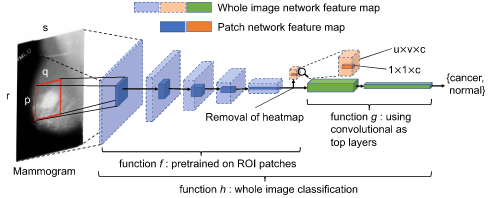
\includegraphics[width=0.8\textwidth]{ML1}
	\caption{Illustration of the pipeline structure \cite{article}}
\end{figure}
\end{frame}


\begin{frame}{Training and Results I}

\begin{columns}
	\begin{column}{0.5\textwidth}
		\begin{itemize}
			\item SBIS-DDSM containing annotated ROIs
			\item Pre-train patch classifier on sample patches
			\item<2-> Test on entire images after fine-tuning second segment
		\end{itemize}
	\end{column}
	\begin{column}{0.5\textwidth}
		\begin{figure}
			
			\centering
			\visible<3>{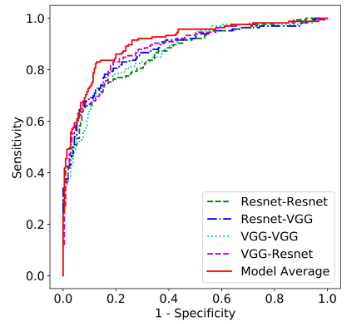
\includegraphics[width=\textwidth]{ML2}}
			%\caption{Illustration of Catastrophic Forgetting \cite{zenke2017continual}}
		\end{figure}
	\end{column}
\end{columns}


\end{frame}
\begin{frame}{Training and Results II}
	\begin{columns}
		\begin{column}{0.5\textwidth}
			\begin{itemize}
				\item Test transferability on INbreast dataset
				\item<2-> Use pre-trained patch classifier from previous training set
				\item<3-> Good results after few images already: Intensive part lies in fine-tuning patch classifier
			\end{itemize}
		\end{column}
		\begin{column}{0.5\textwidth}
			\begin{figure}
				
				\centering
				\visible<3>{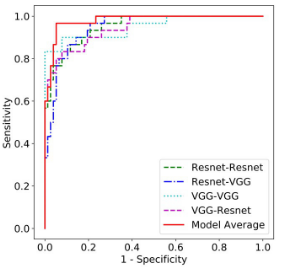
\includegraphics[width=\textwidth]{ML3}}
				%\caption{Illustration of Catastrophic Forgetting \cite{zenke2017continual}}
			\end{figure}
		\end{column}
	\end{columns}
\end{frame}





\section{Discussion}
    \begin{frame}[plain]
        \vfill
      \centering
      \begin{beamercolorbox}[sep=8pt,center,shadow=true,rounded=true]{title}
        \usebeamerfont{title}\insertsectionhead\par%
        \color{oxfordblue}\noindent\rule{10cm}{1pt} 
        
      \end{beamercolorbox}
      \vfill
  \end{frame}
\begin{frame}{Discussion}
  \begin{itemize}
  	\item End-to-end learnable deep learning approach
  	\item<2-> Great versatility due to pipeline structure
  	\item<3-> Still doesn't overcome reliance on labelled ROIs to further increase performance 
  \end{itemize}
\end{frame}



\begin{frame}{References}

\bibliography{References}
\end{frame}
\end{document}

